

%************************************************
\chapter{Proposal}\label{ch:proposal}

%************************************************
\begin{quotation}
	\small \textit{ \flushright
	Everything is theoretically impossible, until it is done.
	\flushright --- Robert A. Heinlein \\
	\vspace{1cm}}
\end{quotation}


This chapter presents the plan for finishing the dissertation.


\section{The tortuous path so far} Before presenting the plan of work for the future, it will be enlightening to describe our journey so far.

From the beginning, the goal has always been to research how to achieve state of the art results in Deep Learning with significantly smaller datasets\footnote{Moacir: ok, but it does not match the text in chap1. }. This goal is one of the most significant challenges of the artificial intelligence community; to democratise deep learning, and prevent that it becomes a game of a handful of influential organisations.

The urge for developing methods for learning with less data became even more pressing as our research group shifted its focus to \acf{NLP}.

\paragraph{Transfer Learning} Thus, we started by researching Transfer Learning (TL). Transfer learning is one of the most critical developments in \acs{DL} and the reason for much of the current success in the field.

In this research of TL, there was an encouragement to do a literature review, which produced the paper~\citeauthoritle{guth:2019}~\cite{guth:2019} (appendix \ref{ch:frontiers}). In this review, it became clear that:
\begin{enumerate}
	\item Transfer learning in NLP was a promising field, with exciting new results like ULMFit~\cite{howard:2018universal} and BERT~\cite{devlin:2018}.
	\item There is an outpace between practice and theory in Deep Learning, and several unexplained phenomena and methods that work well in practice without theoretical support.
\end{enumerate}
The premise, then, was that by studying the theory, it would be possible to have insights on developing new methods to achieve more efficiency in transfer learning and, consequently, need less data. And then, we fell down \emph{the rabbit hole}.
\paragraph{Machine Learning Theory} By trying to understand one of the first papers on the theory of transfer learning (\citeauthor{baxter:2000}), it was evident there was a lack of knowledge in Machine Learning Theory. Understanding the current theory became an effort of several months, and culminated in frustration.

The study of \ac{MLT} explained why the community had turned its back to theory: the current general theory contradicts phenomena experienced in practice and did not guide why methods worked or what is promising.

As we were about to give up the theoretical effort, there was a serendipitous finding: Tishby's video on a new general theory for Deep Learning based on Information Theory~\cite{tishby:2017} started to trend and received positive critiques from widely respected researchers like Geoffrey Hinton and Samy Bengio. And then, another \emph{rabbit hole}.

\paragraph{The Bottleneck theory of deep learning} The study of the Bottleneck theory of deep learning was arduous for several reasons:
\begin{itemize}
	\item It assumed knowledge in Information Theory, which was not the case and took other months.
	\item It is a very new field, and several essential papers were being published as we were doing the literature review.
	\item It is not well established yet, the work is scattered in several papers and still need to be consolidated.
\end{itemize}
From the initial literature review, the technical report~\citeauthoritle{guth:2019transferability}~\cite{guth:2019transferability} (annexed in appendix \cref{ch:transferability}) was produced. Moreover, it was evident that the difficulty found was a great research opportunity.


\section{Proposal} We propose to consolidate the scattered knowledge on the \acf{IBT}in a comprehensive manner.

The literature reviewed so far:
\begin{itemize}
	\item~\citeauthoritle{tishby:2015dlib}~\cite{tishby:2015dlib} ~(\citeauthor{tishby:2015dlib},~\citeyear{tishby:2015dlib})
	\item~\citeauthoritle{shwartz-ziv:2017}~\cite{shwartz-ziv:2017} ~(\citeauthor{shwartz-ziv:2017},~\citeyear{shwartz-ziv:2017})
	\item~\citeauthoritle{achille:2017emergence}~\cite{achille:2017emergence} ~(\citeauthor{achille:2017emergence},~\citeyear{achille:2017emergence})
	\item~\citeauthoritle{zaslavsky:2018}~\cite{zaslavsky:2018} ~(\citeauthor{zaslavsky:2018},~\citeyear{zaslavsky:2018})
	\item~\citeauthoritle{achille:2018critical}~\cite{achille:2018critical} ~(\citeauthor{achille:2018critical}~\citeyear{achille:2018critical})
	\item~\citeauthoritle{achille:2018infodropout}~\cite{achille:2018infodropout} ~(\citeauthor{achille:2018infodropout},~\citeyear{achille:2018infodropout})
	\item~\citeauthoritle{achille:2018dynamics}~\cite{achille:2018dynamics} ~(\citeauthor{achille:2018dynamics},~\citeyear{achille:2018dynamics})
	\item~\citeauthoritle{achille:2019complexity}~\cite{achille:2019complexity} ~(\citeauthor{achille:2019complexity},~\citeyear{achille:2019complexity})
	\item~\citeauthoritle{shwartz-ziv:2019}~\cite{shwartz-ziv:2019} ~(\citeauthor{shwartz-ziv:2019},~\citeyear{shwartz-ziv:2019})
	\item~\citeauthoritle{saxe:2019}~\cite{saxe:2019} ~(\citeauthor{saxe:2019},~\citeyear{saxe:2019})
	\item~\citeauthoritle{achille:2019weights}~\cite{achille:2019weights} ~(\citeauthor{achille:2019weights},~\citeyear{achille:2019weights})
	\item~\citeauthoritle{achille:2019phd}~\cite{achille:2019phd} ~(\citeauthor{achille:2019phd},~\citeyear{achille:2019phd})
\end{itemize}


\section{Schedule}
\paragraph{IBT SotA update} Besides the literature reviewed so far, we will keep checking the state-of-the-art in the Information Bottleneck Theory. This is a background task that may take several months.
\paragraph{Using IBT insights in Research} The study of the Information Bottleneck Theory provided some insights for new research: the relationship of superconvergence and the phase transition between information conversion phase and information forgetting phase; the difference in complexity measures between transfer learning and multitask learning; the evidence of the bottleneck limit in natural languages and its application in automatic language translation; etc. We expect that the research in this area allow us to publish at least one paper in a reputable conference.
\paragraph{Seminars on IBT} As preparation for the dissertation writing, and also as part of our research group effort in knowledge dissimination, seminars on the Information Bottleneck Theory will be presented and open to other students.

%%% to set largefigure as the sum of the
%%% width of the text, of the width of the margin note and
%%% of the width of the white spaces between the thext and
%%% the margin note.
%%
\begin{figure}[ht]
	\centering \makebox[
	\textwidth][r]{

	% %%% you make a box which width is
	%%% not important for the contents of the box itself
	%%% (\textwidth) and which will flush [r] from the right
	%%% ([l] from the left) margin of the text; whatever doesn't
	%%% find place in the box will exceed in the opposite side.
	%%% Please note that a curly brace is still open.

	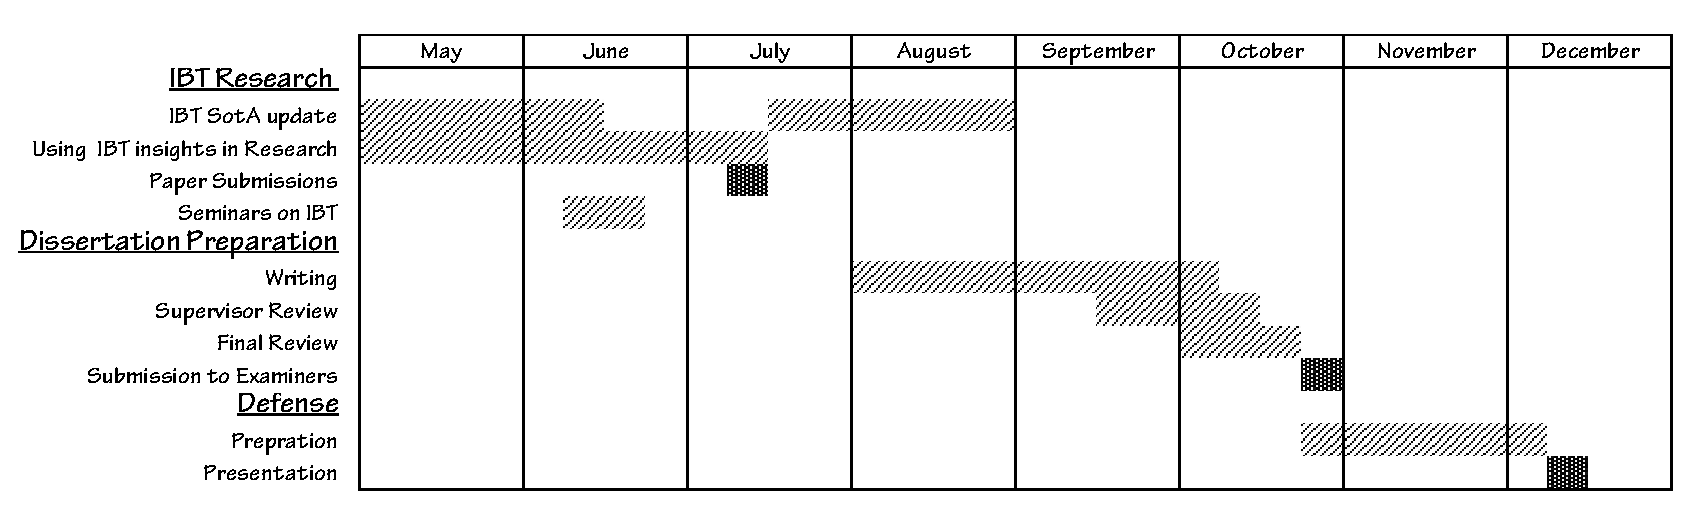
\includegraphics[width=.9\largefigure]{schedule}

	%%% you
	%%% can now include your graphic with the usual option for
	%%% \includegrephics
	}

	%%% Here you "close the box"

	\caption{Work plan for the rest of the dissertation.}
\end{figure}


\section{Final Considerations}

To the extent of our knowledge, this is the first work that consolidates scattered knowledge of this brand new and promising general theory of deep learning in a comprehensive manner.

Its most prominent research contribution is to guide other researchers so that they do not need to take the same tortuous path we took, and facilitate their journey in this brand new promising subfield.

Some of the challenges are to keep pace with the fast development of publications, at the same time, produce original articles and define a clear scope for the writing of the dissertion avoiding new \emph{rabbit holes}.
